Logic-trees are a tool designed to consider in a systematic manner the 
epistemic uncertainties of models and parameters included in a hazard 
analysis.
% ..............................................................................
% . . . . . . . . . . . . . . . . . . . . . . . . . . . . . . . . . . . > Figure
\renewcommand{\psedge}{\ncdiag[armA=0,angleB=180,armB=1cm]}
\begin{figure}[!hb]
\hfill \\
\textcolor{blue01}{\emph{Branch set definition}}: \dotfill Simple Fault 
	Dip Angle \\
\textcolor{blue01}{\emph{Branch set uncertainty type}}: \dotfill 
	Absolute values \\
\textcolor{blue01}{\emph{Applies to}}: \dotfill Simple faults \\
\textcolor{blue01}{\emph{Correlated branches}}: \dotfill Yes \\
\hfill \\
	\centering
	\begin{psTree}[treemode=R,levelsep=*2cm]
			{\Tr{ }}
		\begin{psTree}[treemode=R]{
			\Tr{\parbox[b]{4cm}{ value = 30$^\circ$ 
				\newline weight=w$_1$}}}%
		\end{psTree}%
		\begin{psTree}[treemode=R,treenodesize=1cm]{
			\Tr{\parbox[b]{4cm}{ value = 45$^\circ$ 
				\newline weight=w$_2$}}}%
		\end{psTree}%
		\begin{psTree}[treemode=R]{
			\Tr{\parbox[b]{4cm}{ value = 60$^\circ$ 
				\newline weight=w$_3$}}}%
		\end{psTree}%
	\end{psTree}%
\\ \hfill \\
\caption{An example of branch set used to account for the epistemic 
uncertainties on faults dip angle; in this case each branch contains a value 
of the dip.}
\label{fig:logic_tree_branching_levels}
\end{figure}
% . . . . . . . . . . . . . . . . . . . . . . . . . . . . . . . . . . . < Figure
% ..............................................................................

A logic tree cont\-ains three main elements:
\begin{itemize}
\item Branching Level
\item Branch Set
\item Branch
\end{itemize}
%
A \emph{branching level}, expresses the distance of a given element from the 
root of the logic tree; in the simplest case each branching level corresponds 
to a single type uncertainty (e.g. maximum magnitude). 
Indicatively, we can say that the larger the number of branching levels in a 
logic structure the larger is its complexity.
%
\index{Logic Tree!Branch set}
A \emph{branch set} describes an uncertainty model; for example - as previously 
mentioned - a model accounting for the epistemic uncertainties connected with 
the definition of maximum magnitude. A branch set contains of a number of 
mutually exclusive and collectively exhaustive options \citep{bommer2008}. 
%
Finally, a \emph{branch} represent a particular alternative in a branch set and 
therefore it refers to an uncertainty model and has a weight expressing - 
according to different interpretations available in the literature 
- ``probabilities or simply subjective indications of relative merit'' 
\citep[][page 999]{bommer2008}.
	\index{Logic Tree!Branch}

%
In more detail, a branch set - the fundamental component in our logic tree data 
model - consists on (1) the parameter (or model) affected 
by uncertainty, (2) the specification of the type of uncertainty (3) the 
listing of the - mutually exclusive and collectively exhaustive 
- alternative hypotheses (4) a weight for each hypothesis, 
(5) a flag specifying if the branches are (totally) correlated and, (6) the 
index of the branches of the previous level - or the subset of seismic 
sources - to which this branch set applies.

Figure \ref{fig:logic_tree_branching_levels} depicts a branch 
set fixing epistemic uncertainties on the dip angle of simple 
fault sources. In this case the possible values of the dip are specified
on each branch composing the branch set (i.e. 30, 45 and 60 degrees). This 
means that these three values are the only ones admitted for all the sources 
included in the initial seismic source model considered. 
%
Figure \ref{fig:logic_tree_branching_levels_1} also shows a branch
set defining epistemic uncertainties on the dip angle 
of simple fault sources. In this case, however, the values specified for each 
branch aren't absolute dip angles but instead differential values to be added - 
or subtracted - to the dip value specified for each simple fault source 
contained in the initial seismic sources model.

% ..............................................................................
% . . . . . . . . . . . . . . . . . . . . . . . . . . . . . . . . . . . > Figure
\renewcommand{\psedge}{\ncdiag[armA=0,angleB=180,armB=1cm]}
\begin{figure}
%\fbox{\begin{minipage}{\textwidth}
\hfill \\
\textcolor{blue01}{\emph{Branch set definition}}: \dotfill
	Simple Fault Dip Angle \\
\textcolor{blue01}{\emph{Branch set uncertainty type}}: \dotfill
	Relative values \\
\textcolor{blue01}{\emph{Applies to}}: \dotfill
	All previous branches \\
\textcolor{blue01}{\emph{Correlated branches}}: \dotfill Yes \\
\hfill \\
	\centering
	\begin{psTree}[treemode=R,levelsep=*2cm]
			{\Tr{ }}
		\begin{psTree}[treemode=R]{
			\Tr{\parbox[b]{4cm}{ value = -15$^\circ$ 
				\newline weight=w$_1$}}}%
		\end{psTree}%
		\begin{psTree}[treemode=R,treenodesize=1cm]{
			\Tr{\parbox[b]{4cm}{ value = 0$^\circ$ 
				\newline weight=w$_2$}}}%
		\end{psTree}%
		\begin{psTree}[treemode=R]{
			\Tr{\parbox[b]{4cm}{ value = +15$^\circ$ 
				\newline weight=w$_3$}}}%
		\end{psTree}%
	\end{psTree}%
\\ \hfill \\
%\end{minipage}} % End of fbox
\caption{An example of branch set used to account for the epistemic 
uncertainties on faults dip angle; in this case each branch contains a 
differential from a default dip value indicated for each source in the 
initial seismic sources model.}
\label{fig:logic_tree_branching_levels_1}
\end{figure}
% . . . . . . . . . . . . . . . . . . . . . . . . . . . . . . . . . . . < Figure
% ..............................................................................
Two or more branch sets they can be combined in flexible fashion (i.e. 
concatenated) to create an entire logic-tree structure.
Figure \ref{fig:logic_tree_schema} shows an example of a logic tree 
created by combining the two branch sets described in the upper part of the
figure. 
The first branch set accounts for epistemic uncertainties connected with 
the dip of simple fault sources whilst the second specifies 
the epistemic uncertainties relative to the depth to the top of rupture  
(this branching level also applies to simple faults included in the model).
% ..............................................................................
% . . . . . . . . . . . . . . . . . . . . . . . . . . . . . . . . . . . > Figure
\begin{figure}[!h]
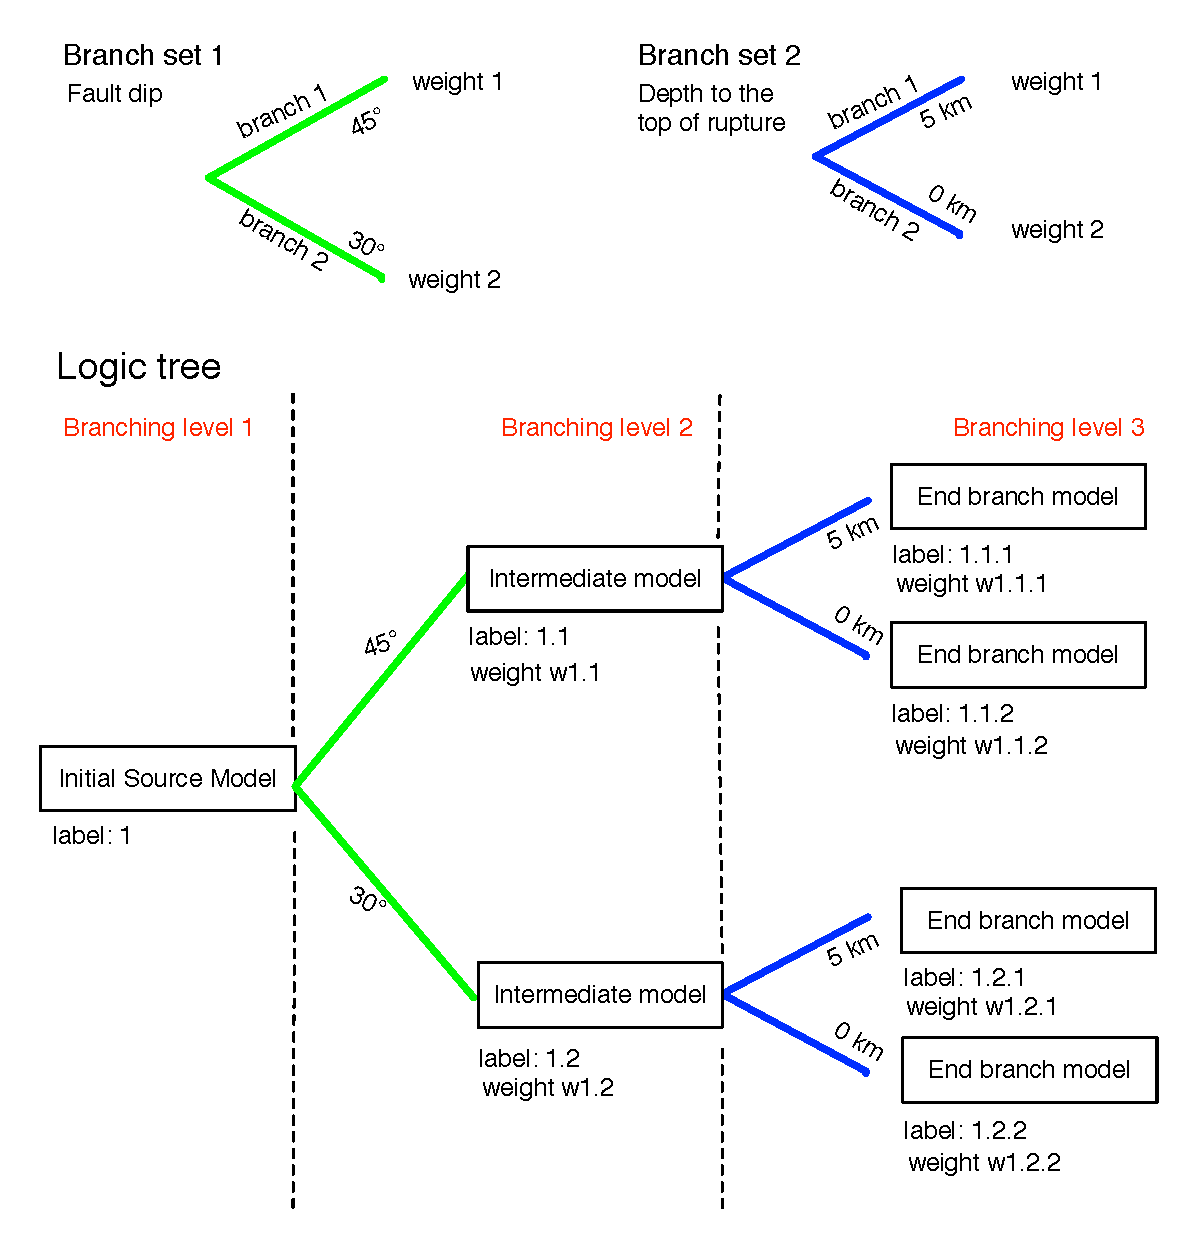
\includegraphics[width=15cm]{./Figures/Part_Hazard/logic_tree_schema.eps}
\caption{Example of a logic tree structure as defined in OpenQuake. The upper
part of the Figure depicts two branch sets.}
\label{fig:logic_tree_schema}
\end{figure}
% . . . . . . . . . . . . . . . . . . . . . . . . . . . . . . . . . . . < Figure
% ..............................................................................
%

This data model permits a very general definitions of logic tree 
structures. For instance, a non-symmetric logic tree can be easily 
created by placing multiple branch sets in the same branching level, each 
branch set being connected to a specific branch of a branch set defined in a
previous branching level. Figure \ref{fig:LogicTreeGeneralStructure}) shows a 
general example of a logic tree structure supported by OpenQuake logic tree 
data model. 

% ..............................................................................
% . . . . . . . . . . . . . . . . . . . . . . . . . . . . . . . . . . . > Figure
\begin{figure}
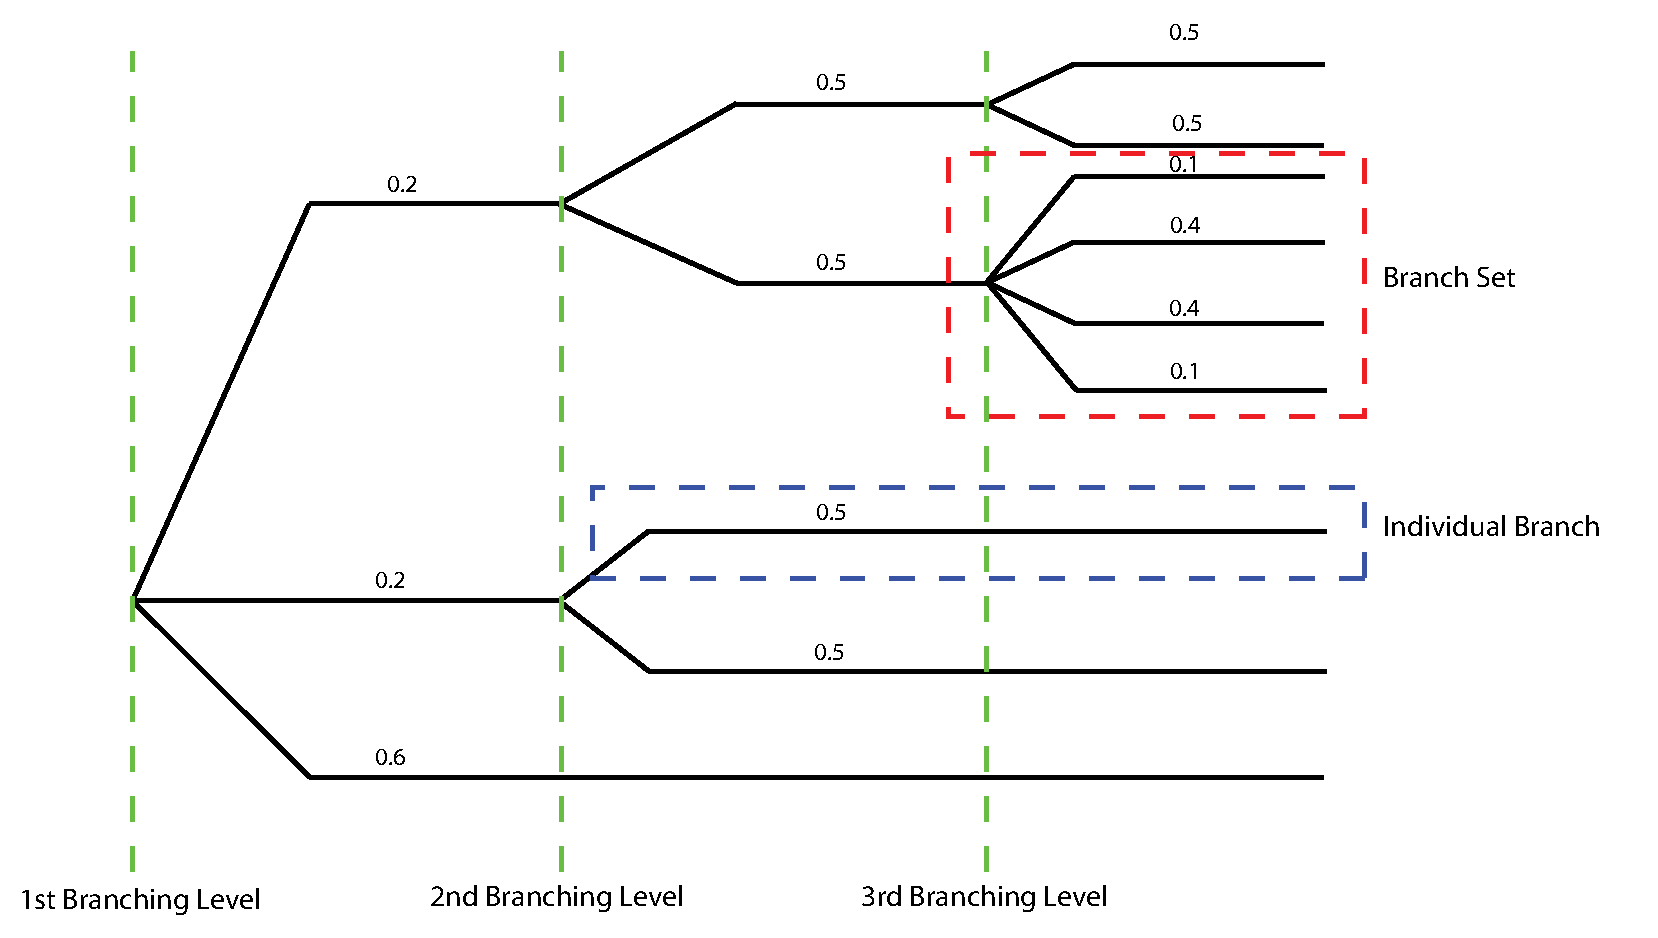
\includegraphics[width=15cm]{./Figures/Part_Hazard/LogicTreeGeneralStructure.eps}
\caption{Logic Tree data structure as defined in terms of individual branches, 
branch sets, and branching levels.}
\label{fig:LogicTreeGeneralStructure}
\end{figure}
% . . . . . . . . . . . . . . . . . . . . . . . . . . . . . . . . . . . < Figure
% ..............................................................................

We use this logic tree description to specify the structure of the Seismic 
Sources Logic Tree as well as for the Ground Motion Logic Tree. 